

\chapter{Metodologia}
\label{ch:Metodologia}

Neste capítulo são descritas as etapas de desenvolvimento do projeto que já foram implementadas, tendo em vista a proposta apresentada para construção de um produto de tecnologia assistiva para ensino de tipografia a deficientes visuais, mais especificamente, do sistema de classificação de tipografias.

O processo de desenvolvimento do sistema se deu em três etapas principais, que são listadas a seguir:

\begin{enumerate}
\item Estruturação do projeto;
\item Composição do banco de dados (imagens das diversas tipografias);
\item Implementação do algoritmo para classificação das imagens.
\end{enumerate}
%\ldots - reticencias

A primeira etapa deste trabalho foi caracterizada por debates para a idealização do produto final de tecnologia assistiva oferecido ao deficiente visual. A segunda e a terceira etapas, por sua vez, foram desenvolvidas e aprimoradas simultaneamente. O processo de desenvolvimento adotado nessas etapas é explicitado abaixo.

Todos os algoritmos implementados para este projeto, bem como o banco de imagens, podem ser encontrados no \textit{link}: \textit{github.com/fegvilela/TCC2}.

%Os resultados dessa etapa foram descritos no capítulo 2, como fundamentação teórica, e no capítulo 1, como apresentação da proposta de projeto. Porém, tópicos em relação ao projeto final do produto encontram-se na seção destinada a trabalhos futuros.
\section{Estruturação do Projeto}

Como primeiro estágio de desenvolvimento do projeto, foram discutidos modelos para a estruturação do produto e realizadas pequenas entrevistas não-estruturadas com deficientes visuais, sendo eles possíveis usuários do produto ou não.

Em oportunidades de teste, descritos e implementados no trabalho de Cruz \citeC{cruz2017}, para aperfeiçoamento das peças táteis no desenvolvimento do produto, também foram realizadas as entrevistas com os deficientes visuais. O foco dessas entrevistas foi o maior entendimento sobre o contato real dos deficientes com o computador e com a informática. Nestas ocasiões, foram questionados aspectos sobre os leitores de tela disponíveis no contexto brasileiro, além de a popularização do sistema operacional \textit{DOSVOX}. O objetivo dessas questões foi direcionar o desenvolvimento futuro do sistema, para que ele seja adaptado às condições reais de tecnologia dos deficientes visuais brasileiros. Além disso, houve a apresentação da proposta do sistema, a qual foi avaliada positivamente.

Vale ressaltar que o contato realizado com estes deficientes visuais foi importante para a idealização e desenvolvimento do projeto até o momento, sendo um vínculo importante para o seguimento deste posteriormente.

\section{Composição do Banco de Imagens}

Passando-se então para as etapas de implementação do sistema, como já descrito, foram escolhidas nove tipografias para o projeto e, para cada uma delas, construído um conjunto de imagens. Para melhor organização, o banco foi montado tipografia a tipografia. As imagens que compõem o banco de dados em sua versão final são caracteres separados de cada tipografia, amostras podem ser vistas na Figura \ref{fig:nimage}.


A principal fonte de obtenção das imagens originais foi o \textit{Fonts in Use}, um website que disponibiliza fotografias de projetos envolvendo design gráfico que já estão classificadas por tipografia \citeC{fontsinuse2017}. Além deste, foram utilizados sites de busca convencionais, utilizando a opção de imagens nas buscas. Ainda, para os casos em que poucas imagens foram encontradas, a saber as tipografias \textit{Franklin Gothic} e \textit{Adobe Jenson}, imagens complementares foram cedidas como cortesia pela estudante de design parceira neste projeto.


\begin{figure}[H]
  \centering
  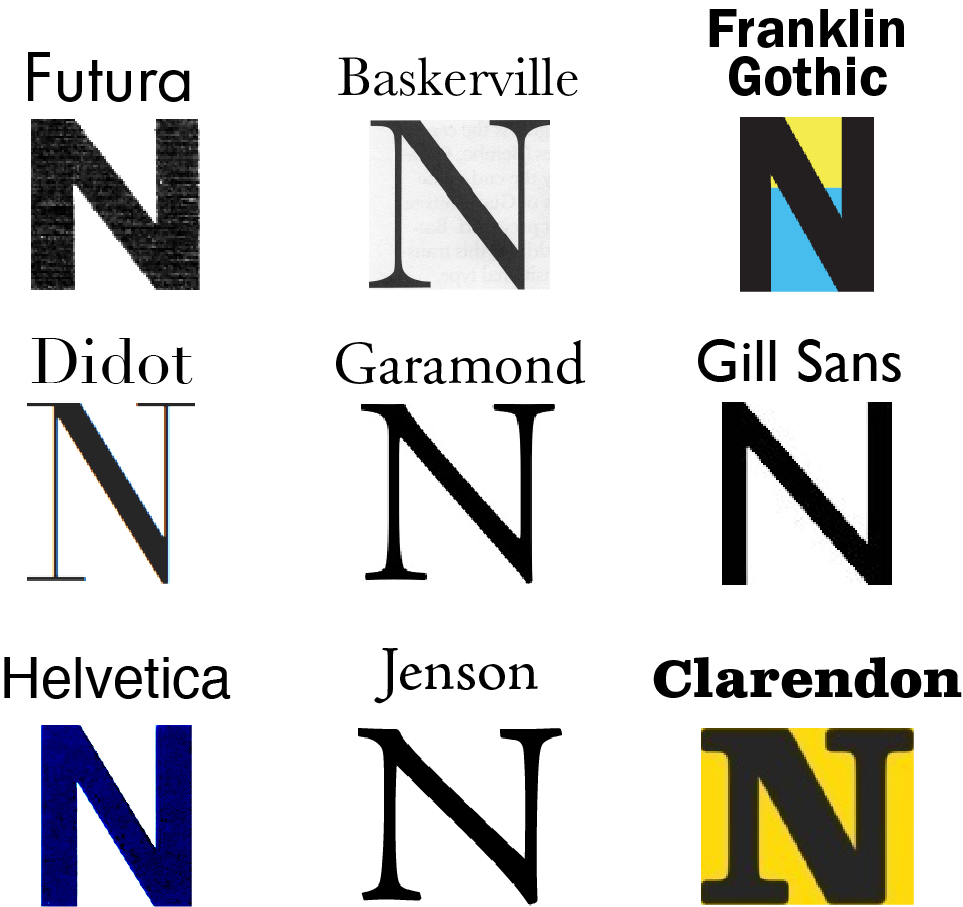
\includegraphics[width=0.4\linewidth]{figuras/nimage.pdf}
  \caption{Amostras do banco de imagens, especificando-se a tipografia.}
  \label{fig:nimage}
\end{figure}


É comum que tipografias digitais apresentem várias versões distintas entre si. Uma vez que as tipografias digitais são representações da versão física original dos tipos, diversas fundidoras de tipos propõem seu próprio modelo representativo para aquela tipografia, ocasionando em variações nas versões digitais. Um exemplo utilizando a tipografia \textit{Garamond} é apresentado na Figura \ref{fig:comparacaoTipos}. Escolheu-se, para ilustração, a letra "a", sendo possível verificar as diferenças no formato de três partes específicas da letra: bojo, remate e terminal em gota. A versão adotada no projeto é a \textit{Adobe Garamond Pro}. Logo, antes de adquirirmos imaens deste tipo em websites, foi necessária uma análise manual para verificar se a imagem se tratava da tipografia correta, em sua versão empregada no projeto.


\begin{figure}[h!]
  \centering
  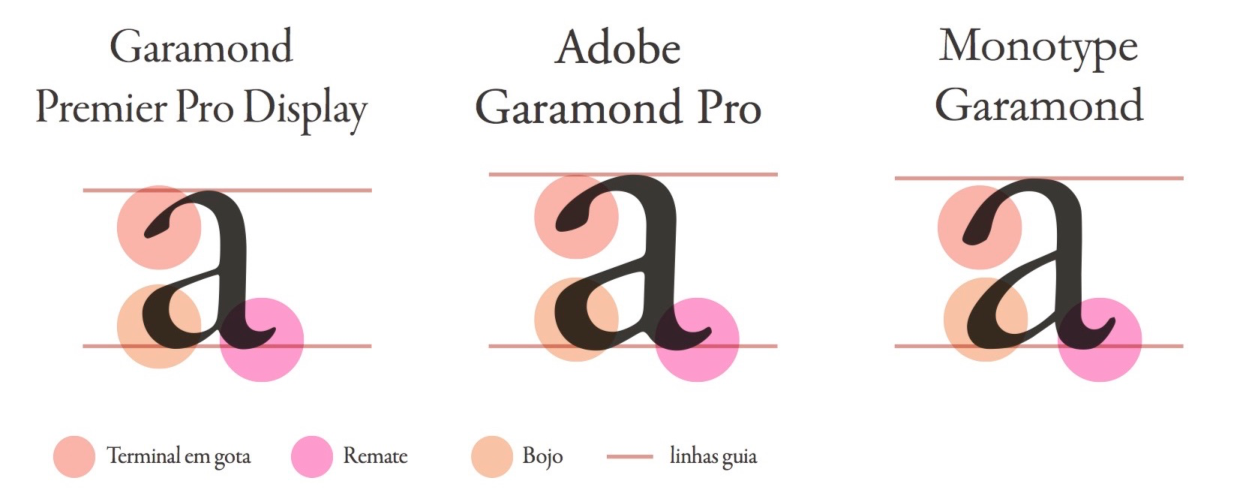
\includegraphics[width=0.65\linewidth]{figuras/comparacaoTipo.pdf}
  \caption{Comparação entre três versões da fonte Garamond, evidenciando as partes anatômicas distintas.}
  \label{fig:comparacaoTipos}
\end{figure}

Sendo assim, a adição de uma imagem de uma outra versão da tipografia poderia gerar um erro de classificação, já que algumas tipografias empregadas no projeto são similares entre si, fato ilustrado na Figura \ref{fig:comparacaoJensonGaramond} que apresenta a similaridade entre duas tipografias presentes no projeto. Portanto, a análise foi realizada de forma minuciosa, utilizando conceitos da anatomia das letras, como o formato de suas serifas e o contraste entre as partes \citeC{rocha2004}. Ademais, as imagens originais obtidas muitas vezes continham variações que deveriam ser excluídas manualmente, como mais de uma tipografia em sua composição, ou então uma mistura entre os variados estilos dentro de uma família tipográfica: itálico, algumas variações de negrito e versalete.

\begin{figure}[H]
  \centering
  
\includegraphics[width=0.4\linewidth]{figuras/comparacaoJensonGaramond.pdf}
  \caption{Comparação entre as fontes \textit{Adobe Garamond Pro} e \textit{Adobe Jenson Pro}, atestando o alto índice de similaridade entre elas.}
  \label{fig:comparacaoJensonGaramond}
\end{figure}

Para o processo de separação das imagens em caracteres únicos, implementou-se um algoritmo em Python para automatização do processo de reconhecimento da localização dos caracteres na imagem e de formação de novas imagens individuais, algo similar a "recortes" {} da imagem original. A principal biblioteca utilizada nesse algoritmo foi a \textit{OpenCV} (\textit{Open Source Computer Vision Library}), uma biblioteca de visão computacional e aprendizado de máquina disponível em código livre (\textit{open source}). Ela foi escolhida por ser amplamente utilizada por especialistas da área e em empresas renomadas como Google, Microsoft, Intel e IBM \citeC{opencv2017}.

O algoritmo desenvolvido é composto de uma seção principal denominada \texttt{mainBancoDados}, e de módulos importados, que incluem os métodos (estruturas em Python análogas à funções) implementados para desempenhar operações específicas nas imagens. O fluxograma do código é ilustrado na Figura \ref{fig:flowMain}. Ao executar o algoritmo, deve-se escolher em qual parte do banco de dados, ou seja, qual tipografia, deseja-se analisar. A seção principal dá acesso à execução de três operações (métodos implementados nesse projeto): recorte das imagens originais, exclusão das imagens de dimensão pequena e renomeação das imagens.

Inicia-se com a aplicação da operação de recorte de imagens (o método \texttt{imCrop}) caso as imagens não sejam letras individuais. Então, caso haja erro no reconhecimento das letras, sendo formada alguma imagem que não apresenta um único caractere por completo, passa-se para o método de exclusão de imagens (\texttt{imApaga}). Em seguida, utilizando o método \texttt{changeName}, realiza-se a renomeação das imagens, caso elas não possuam o nome adequado.

 Vale ressaltar que a formatação padrão para o nome das imagens foi escolhida como: \textit{numero\_tipografia}. Por exemplo, o nome da sétima imagem presente no diretório da tipografia \textit{Helvetica} será "7\_helvetica". O caractere "\_" {} foi escolhido nesse caso para que a classe da imagem, a tipografia, seja de fácil identificação pelo algoritmo de treinamento do modelo classificador.


\begin{figure}[h!]
  \centering
  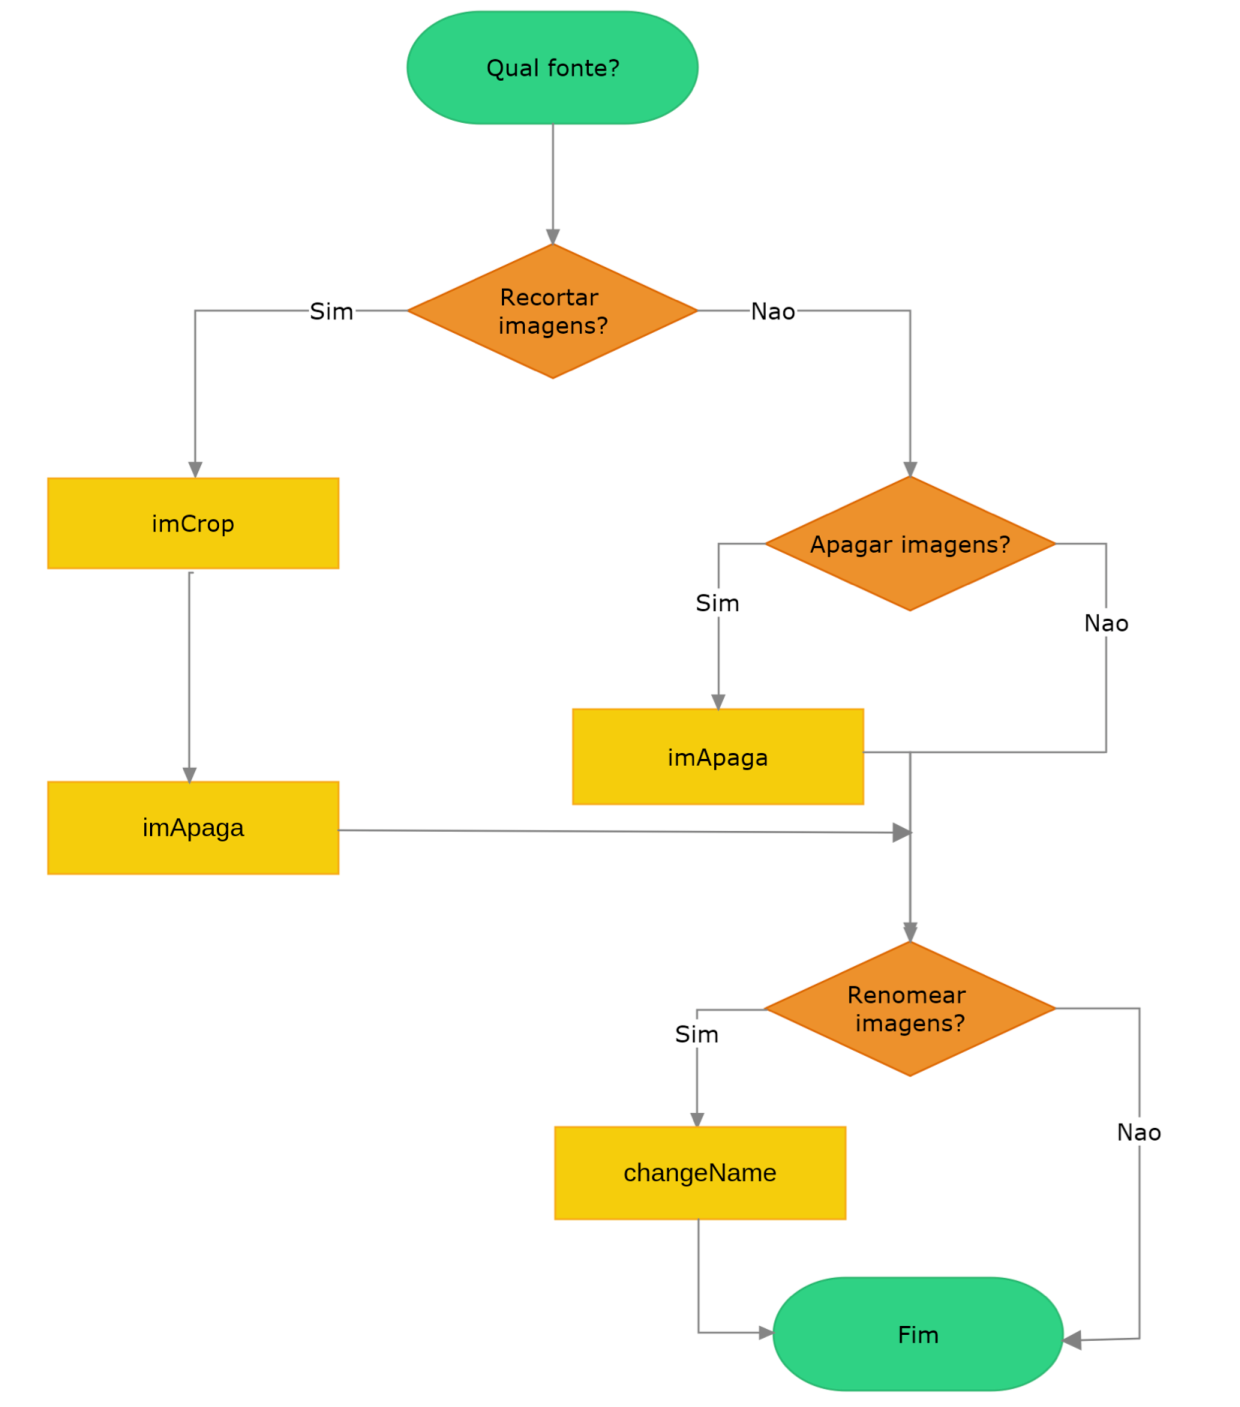
\includegraphics[width=0.9\linewidth]{figuras/mainbancodados.pdf}
  \caption{Fluxograma da seção principal do algoritmo para composição do banco de dados}
  \label{fig:flowMain}
\end{figure}

Passa-se, então, para a descrição de cada um desses métodos separadamente. Em primeiro lugar, o método \texttt{imCrop} realiza o recorte das imagens originais, criando imagens individuais de caracteres. O fluxograma está apresentado na Figura \ref{fig:flowimCrop}. Quando chamado na seção principal, o método \texttt{imCrop} recebe como parâmetro de entrada o nome da fonte em que se deseja operar, já que o banco de imagens é dividido por tipografias. Então, o diretório de operação passa a ser o banco de imagens da fonte escolhida. Todas as imagens contidas naquele diretório são convertidas para o formato \textit{PNG}, que é um dos formatos aceitos pela biblioteca \textit{OpenCV}.


\begin{figure}[H]
  \centering
  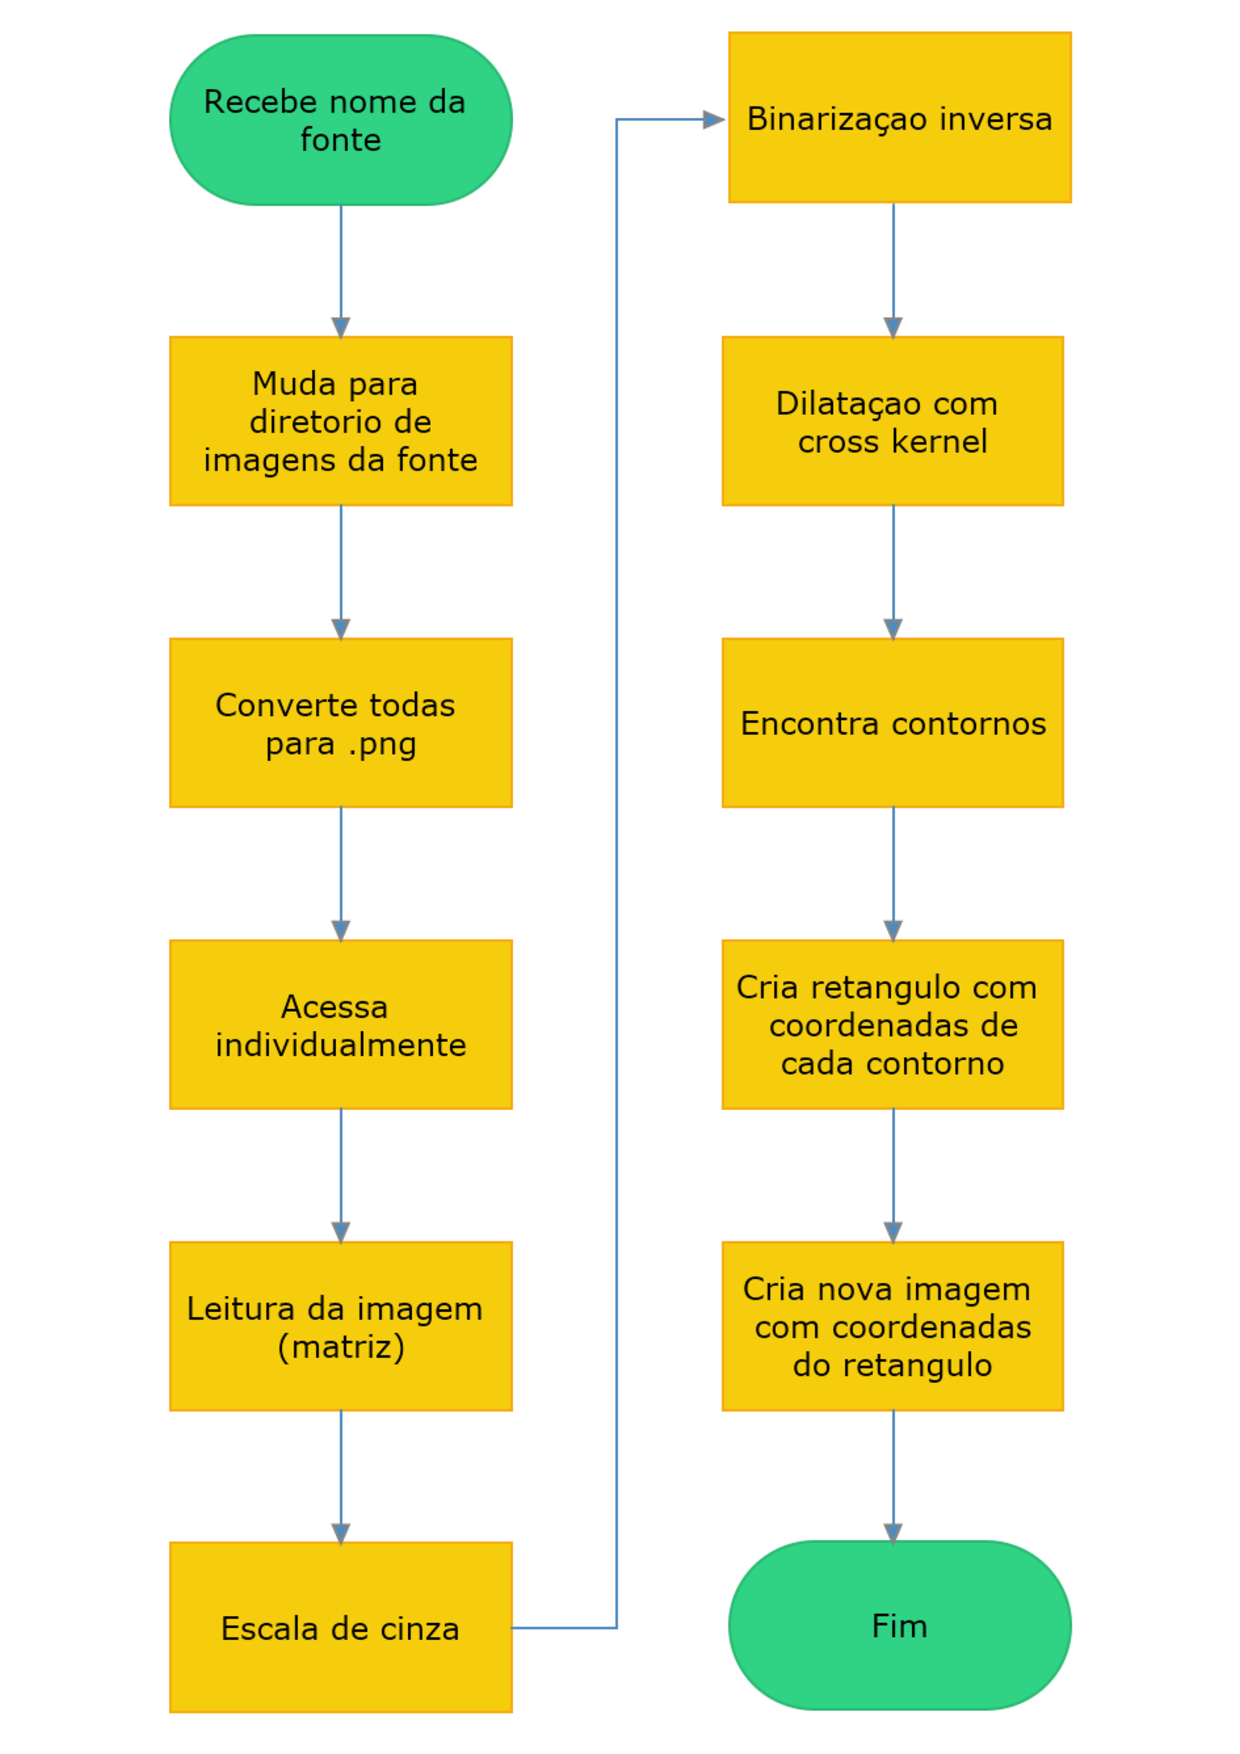
\includegraphics[width=0.6\linewidth]{figuras/imCrop.pdf}
  \caption{Fluxograma do método \texttt{imCrop} para recortar as imagens originais, criando imagens separadas de cada caractere.}
  \label{fig:flowimCrop}
\end{figure}

As imagens são acessadas individualmente e lidas uma por vez. Os valores dos pixels de uma imagem são armazenados em uma matriz. A imagem colorida é convertida para níveis de cinza e, em seguida, é realizada a binarização inversa da imagem em tons de cinza, utilizando um limiar de nível 88, ou seja, valores acima de 88 são atribuídos como valor zero (preto) e valores abaixo, como valor unitário (branco). O próximo passo é a dilatação morfológica usando um \textit{kernel} em cruz, com dimensão 3x3. Após isso, encontram-se os contornos de cada parte branca da imagem. São criados retângulos limitadores ao redor dessas partes da imagem, utilizando as coordenadas dos contornos e novas imagens são criadas a partir desses retângulos. Todo o processo é exemplificado na Figura \ref{fig:imProcess} para uma imagem da fonte \textit{Futura}.



Vale ressaltar que, por envolver um processo de binarização inversa no algoritmo, não foi possível efetuar a detecção de borda nas letras das imagens que, em escala de cinza, possuíam cor de fundo com tom mais escuro que aquele da letra. Portanto, se fez necessária uma correção na coloração de algumas imagens para melhor desempenho do algoritmo, processo realizado manualmente, no software \textit{Pré-Visualização} do sistema operacional \textit{Mac OS X} e também no software \textit{Adobe Lightroom}. Além disso, em algumas imagens, as letras em texto encontravam-se muito próximas uma à outra, o que gerou a demanda de uma limpeza de partes residuais de outras letras, após a formação das imagens de caracteres individuais.

\begin{figure}[H]
  \centering
  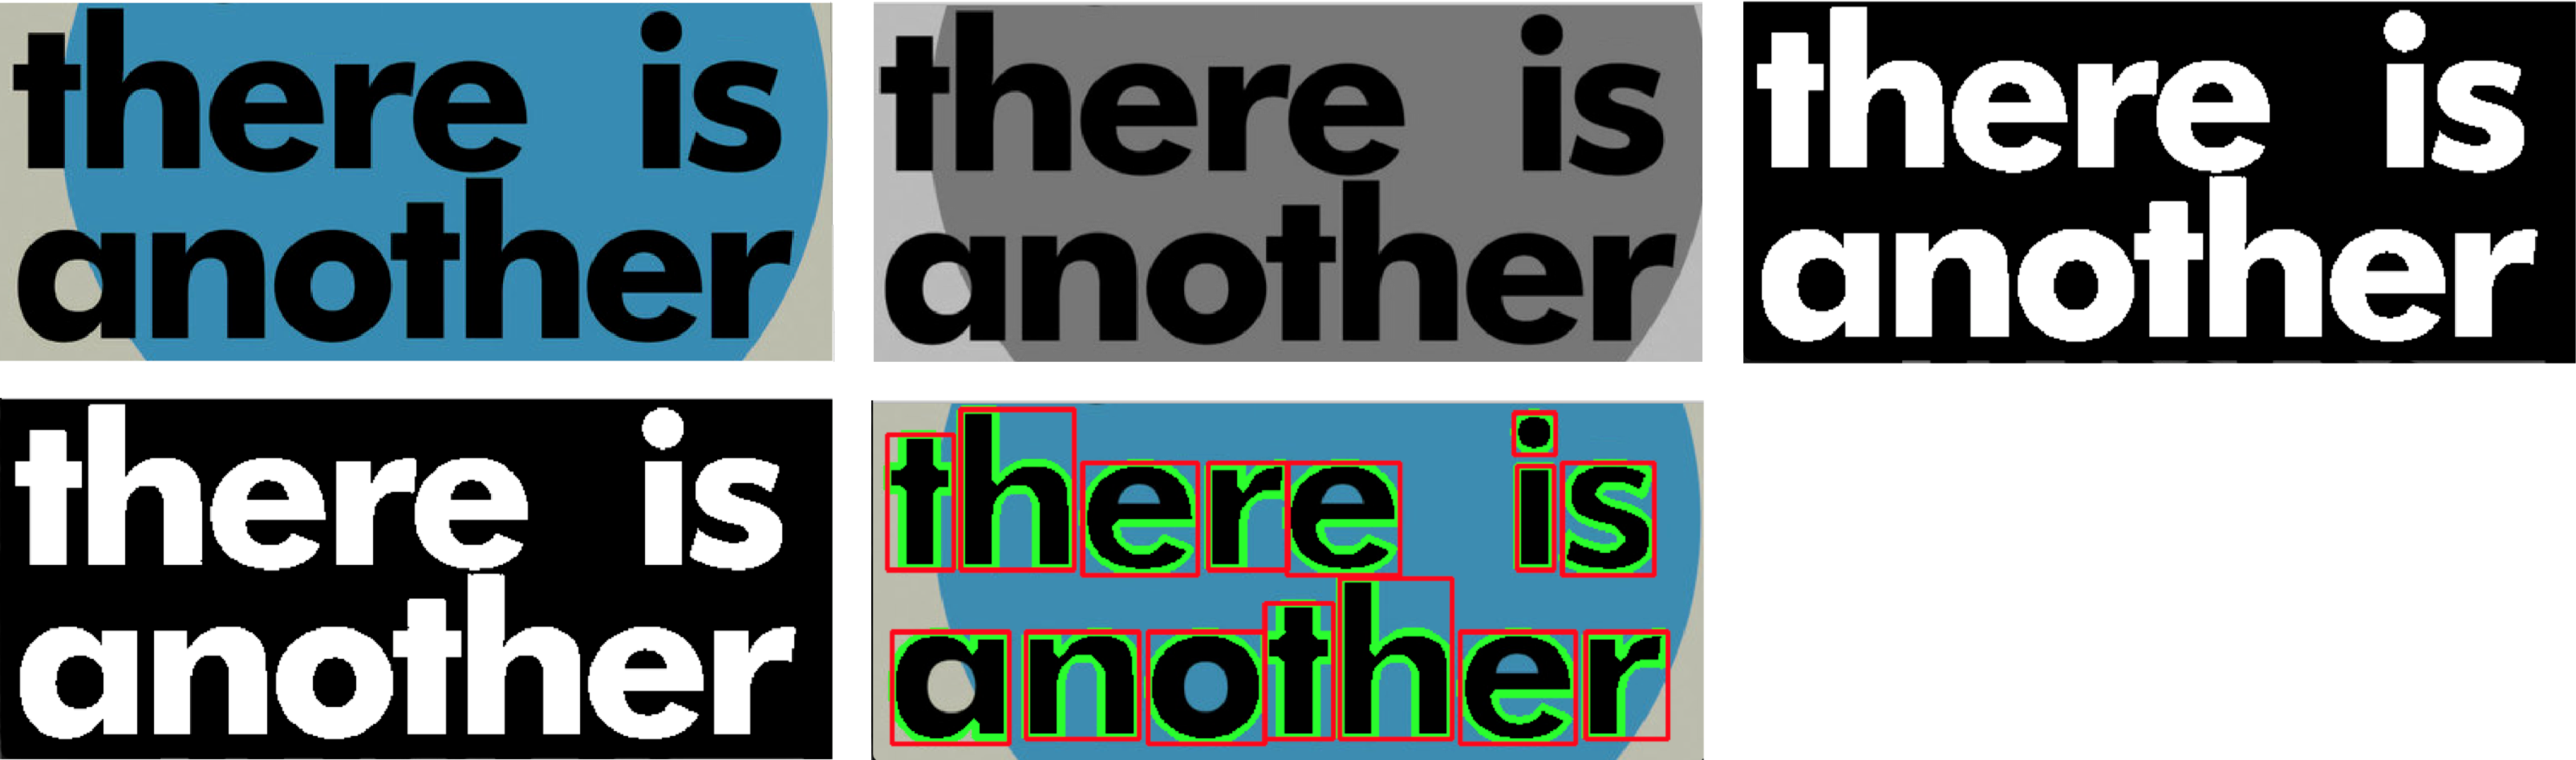
\includegraphics[width=0.9\linewidth]{figuras/imProcess2.pdf}
  \caption{Resultado por etapa do processo de reconhecimento de caracteres em imagens do banco de imagens. i)imagem original, ii)escala de cinza, iii)binarização inversa, iv)dilatação com \textit{kernel} em cruz e v)contornos e retângulos limitadores}
  \label{fig:imProcess}
\end{figure}

O próximo método utilizado na seção principal do algoritmo é \texttt{imApaga}, responsável por excluir as imagens que possuem ambas dimensões inferiores a 45 pixels. O fluxograma descritivo pode ser visto na Figura \ref{fig:flowimApaga}.


\begin{figure}[H]
  \centering
  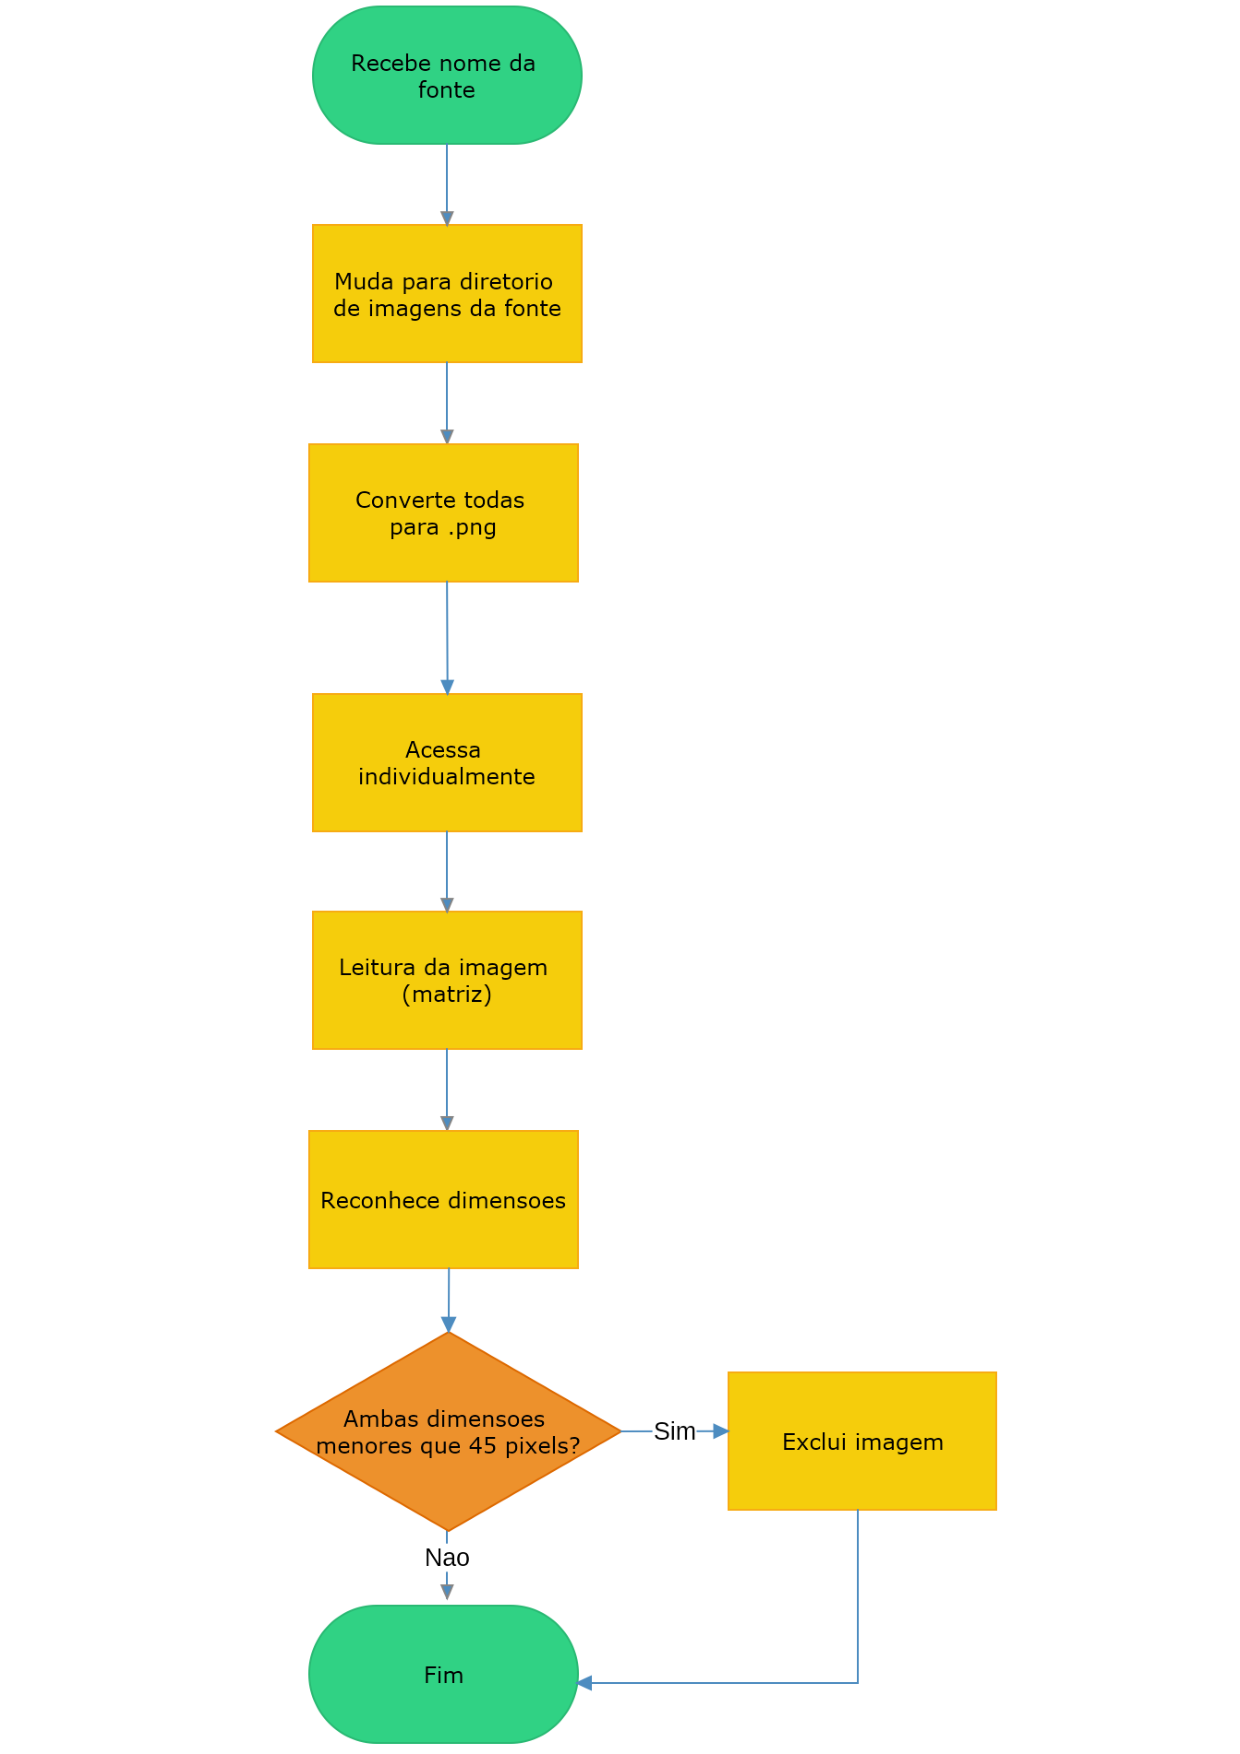
\includegraphics[width=1\linewidth]{figuras/imApaga.pdf}
  \caption{Fluxograma do método \texttt{imApaga} para excluir imagens com dimensões pequenas}
  \label{fig:flowimApaga}
\end{figure}

Assim como no método \texttt{imCrop}, recebe-se como parâmetro de entrada o nome da tipografia em que se deseja operar e muda-se para o diretório do banco de imagens da tipografia. Faz-se também a conversão de todas imagens para \textit{PNG}, que são depois acessadas individualmente e lidas, armazenando as intensidades dos pixels em uma matriz. Após isso, as dimensões da imagem são reconhecidas e avaliadas. Caso as duas dimensões sejam menores que 45 pixels, a imagem é excluída. Caso contrário, o programa passa para a próxima imagem, até finalizar a análise de todas as imagens presentes naquele diretório.

Por sua vez, o método \texttt{changeName} é utilizado para renomear as imagens presentes no diretório de acordo com a tipografia a que pertencem, seguindo o padrão estabelecido para o projeto (\textit{numero\_tipografia}). O fluxograma desse método é apresentado na Figura \ref{fig:flowchangeName}. Assim como os demais métodos dessa seção, começa-se recebendo o nome da tipografia em qual se deseja operar e transfere-se para o diretório do banco de imagens dessa tipografia.

A biblioteca (\textit{OS}) em \textit{Python} utilizada nesse método para a renomeação de arquivos pode gerar um problema durante o processo. Caso o novo nome escolhido para renomear um arquivo seja pertencente a um outro arquivo já existente no diretório, este arquivo prévio é excluído. Portanto, para evitar que arquivos sejam excluídos erroneamente apenas por receberem nomes repetidos, primeiramente verifica-se se há o caractere "\_" {} no nome dos arquivos. Caso negativo, utiliza-se a nomenclatura padrão supracitada, pois, dessa forma, não existirá arquivos prévios com nomenclatura semelhante a essa (\textit{numero\_tipografia}). Porém, caso a verificação apresente resultado positivo, nomeiam-se todos os arquivos com nomenclatura sem o caractere "\_" {}. Esse processo é realizado para garantir que, naquele diretório, nenhuma imagem possui a nomenclatura padrão, prevenindo-a de ser excluída. Então, posteriormente, utiliza-se a nomenclatura padrão em segundo processo automático de renomeação.


O banco de imagens, em versão final, constitui-se de 6750 imagens no total, sendo 750 imagens por tipografia, com dimensão mínima de 45 pixels em altura ou largura. No entanto, inicialmente, para as primeiras quatro tipografias, o banco contava com 1895 imagens para cada uma delas. Porém, muitas imagens possuiam dimensão pequena, apresentando baixa resolução e ruídos, fato que comprometia o treinamento e, consequentemente, a acurácia do classificador. Sendo assim, decidiu-se reduzir o tamanho do banco de imagens, exluindo automaticamente aquelas que fossem menor do que a dimensão desejada. Além disso, em alguns casos, aprouve-se operar uma exclusão manual de imagens provenientes de erros de reconhecimento realizado pelo algoritmo ou que apresentavam baixa resolução, apesar de dimensão maior do que 45 pixels.


\begin{figure}[H]
  \centering
  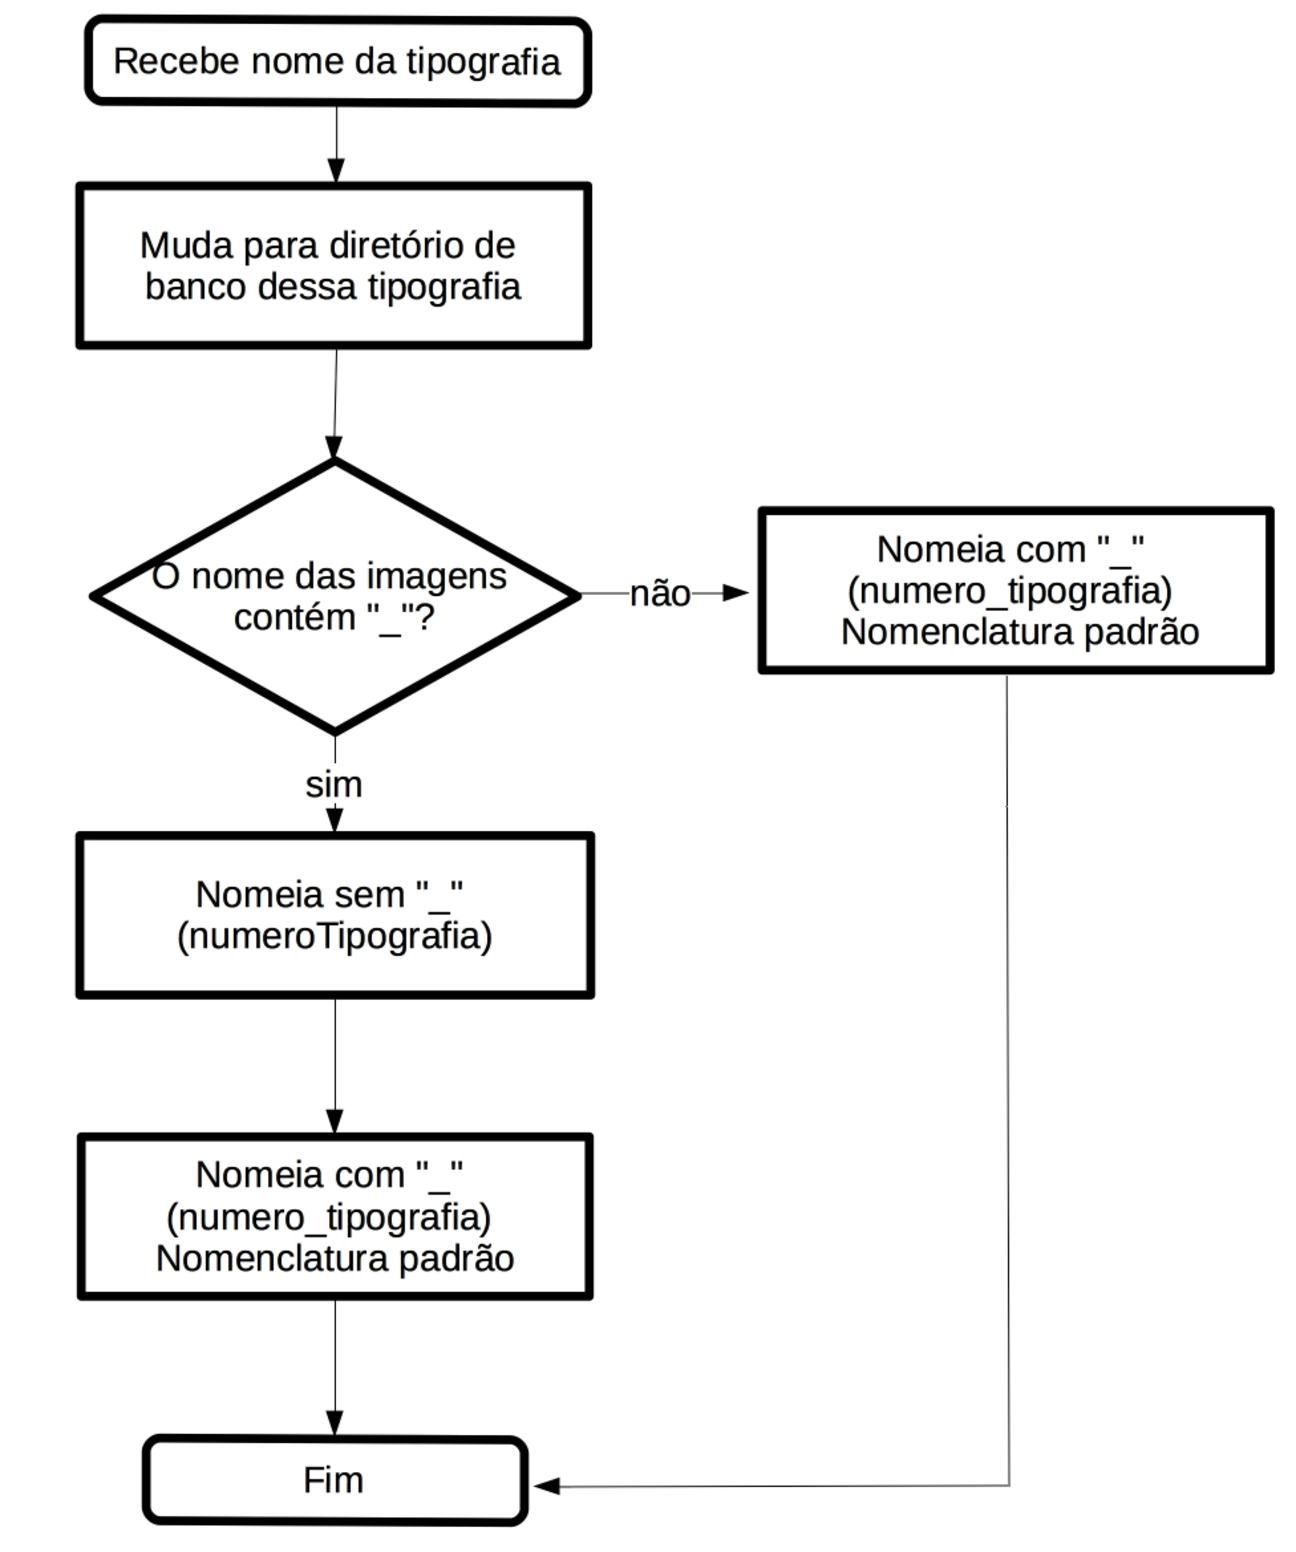
\includegraphics[width=0.55\linewidth]{figuras/changeName.pdf}
  \caption{Fluxograma do método \texttt{changeName} para renomear imagens de determinado diretório, preparando-as para o treinamento do modelo.}
  \label{fig:flowchangeName}
\end{figure}

%O processo de composição do banco de imagens para o treinamento do modelo a ser empregado na máquina foi a parte que mais demandou tempo em todo o processo de desenvolvimento do software. No entanto, em projetos nos quais a aprendizagem de máquina é utilizada essa etapa costuma ser descrita como demorada, como por exemplo (referência).


\section{Algoritmo para Treinamento do Modelo}

Essa seção destina-se à descrição do algoritmo implementado para treinamento do modelo da máquina, bem como das ferramentas utilizadas para seu desenvolvimento. O algoritmo é composto de três estágios listados a seguir, sendo que o resultado de um é o dado de entrada para o estágio subsequente:

\begin{enumerate}
\item Pré-processamento;
\item Extração de atributos;
\item Treinamento do modelo classificador e testes de predição.
\end{enumerate}

Vale ressaltar que as etapas de pré-processamento e de extração de atributos são consecutivas e feitas imagem a imagem, até que todas as imagens do banco sejam avaliadas. Sendo assim, uma imagem passa pelo estágio de pré-processamento, em seguida, pelo estágio de extração de atributos, para que, então, siga-se para a próxima imagem, realizando o mesmo processo.

O algoritmo foi também implementado em Python utilizando como bibliotecas principais o \textit{SciKit-learn}, o \textit{SciKit-image}, o \textit{NumPy} e o \textit{OpenCV}. Todas as bibliotecas citadas, exceto a \textit{OpenCV}, são derivadas de uma só coleção de bibliotecas, denominada \textit{SciPy}, que apresenta softwares de código livre para computação científica em Python. No entanto, as bibliotecas \textit{SciKit}, abreviação de \textit{SciPy Toolkits}, são pacotes complementares ao \textit{SciPy}, sendo desenvolvidas independentemente. O motivo de escolha dessas bibliotecas foi que eles são amplamente utilizados na área de processamento de imagens e aprendizado de máquina \citeC{skimage2014}  \citeC{sklearn2011} \citeC{scipy2017} \citeC{numpy2017}.

\subsection{Estágio de pré-processamento}

Para essa etapa, a principal biblioteca utilizada foi o  \textit{OpenCV}, com a qual foi implementado um processo similar ao método \texttt{imCrop} descrito na seção anterior. Todos os passos do pré-processamento encontram-se ilustrados na Figura \ref{fig:flowpreProc}.

\begin{figure}[h!]
  \centering
  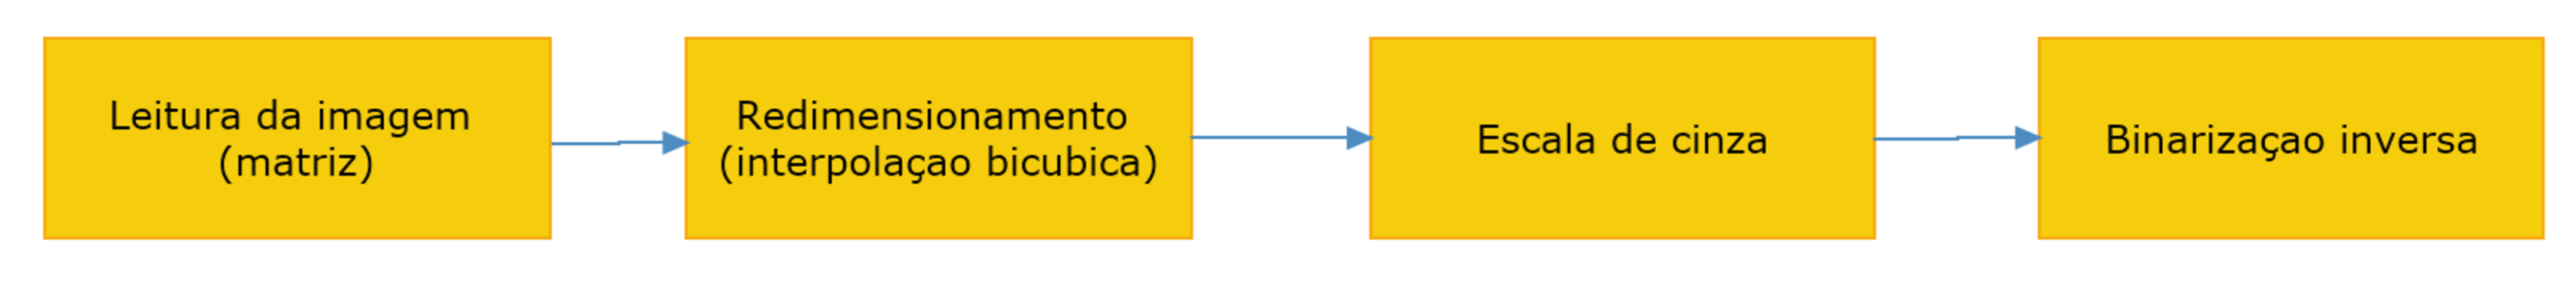
\includegraphics[width=1\linewidth]{figuras/preprocess.pdf}
  \caption{Etapas do estágio de pré-processamento do algoritmo de treinamento do modelo.}
  \label{fig:flowpreProc}
\end{figure}

Inicia-se pela leitura da imagem, transformando-a em matriz, seguido de seu redimensionamento por interpolação bicúbica para altura fixa de 126 pixels, garantindo, assim, uma melhor uniformidade das imagens para o processo de extração de atributos. O valor ótimo da nova dimensão foi encontrado por meio de iterações e testes de acurácia. Para esse teste, criou-se um \textit{loop} para alterar o valor da nova dimensão das imagens e, para cada valor de dimensão, o modelo era treinado e avaliada a acurácia. Desta forma, escolheu-se a dimensão que proporcionou maior acurácia. Posteriormente, a imagem é convertida para escalas de cinza e, por fim, é realizada uma binarização inversa da imagem.

 %Todo esse processo é demonstrado como exemplo na Figura X.

%\begin{figure}[H]
%  \centering
%  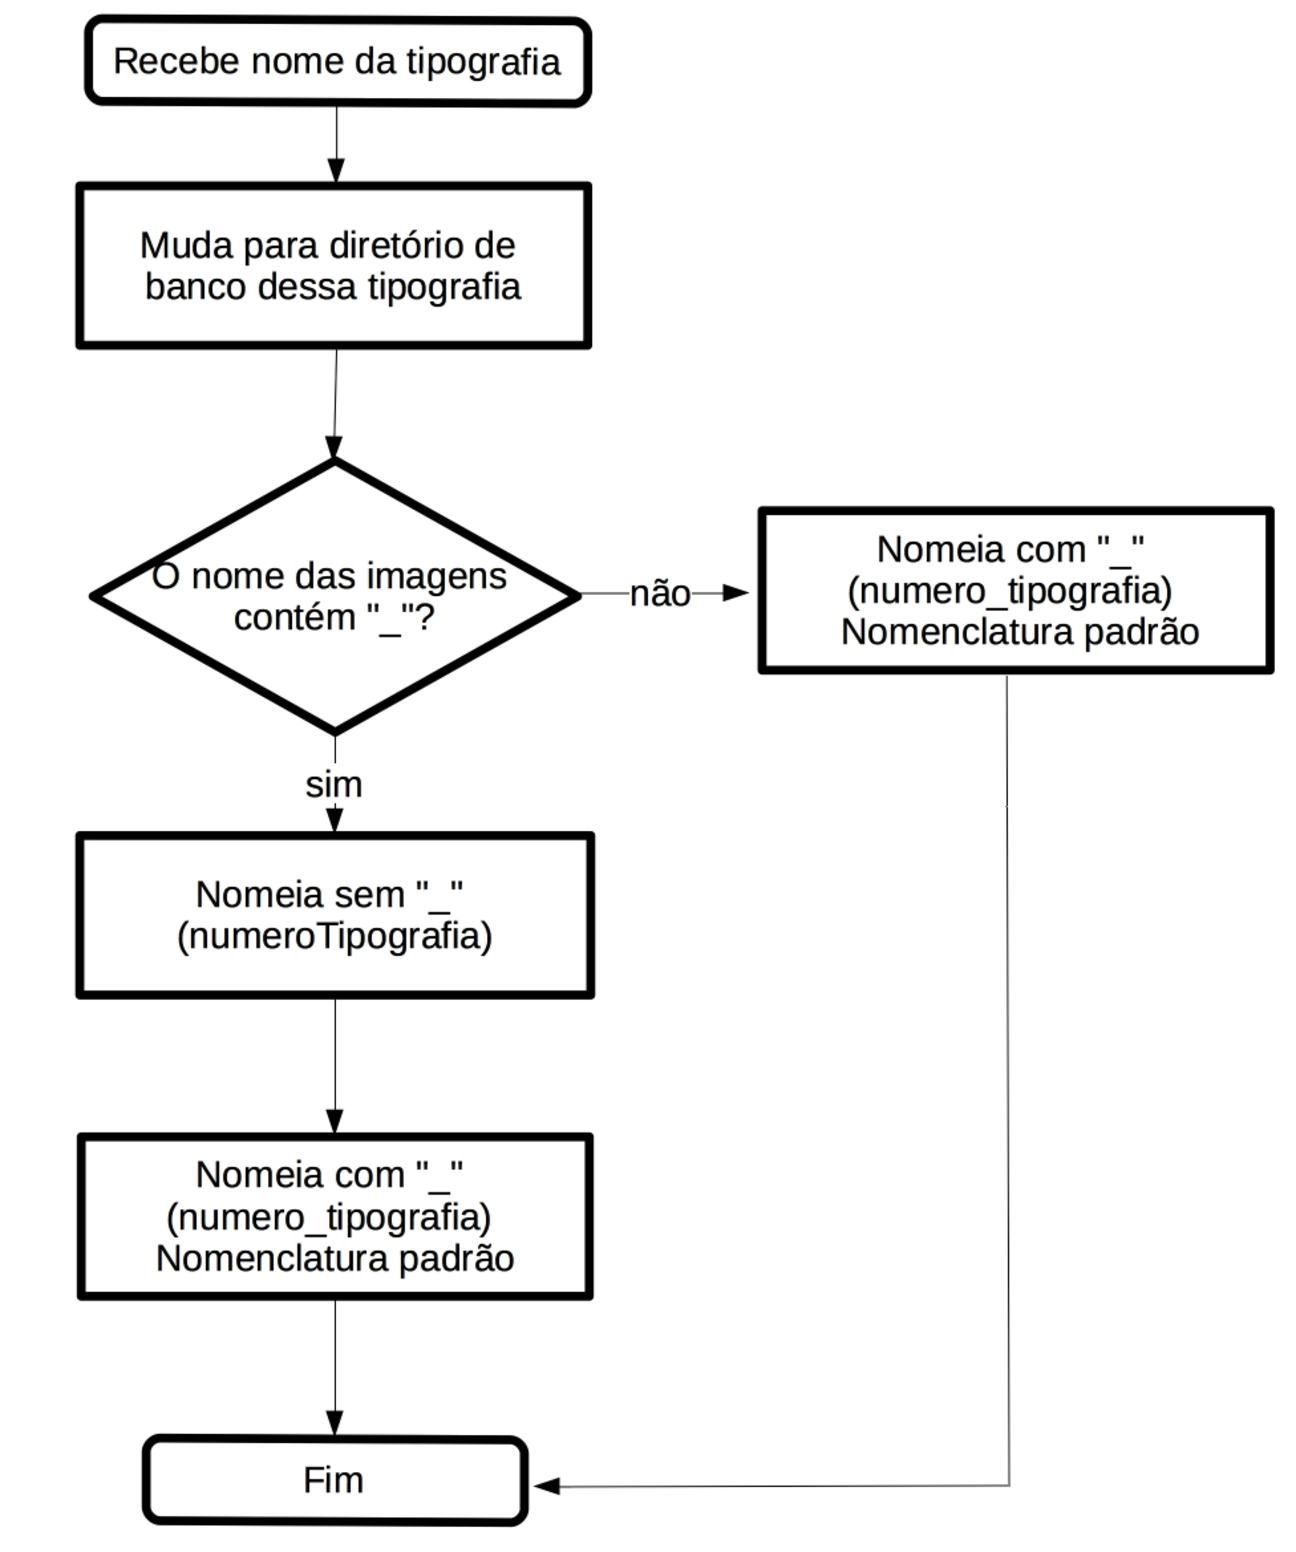
\includegraphics[width=0.6\linewidth]{figuras/changeName.pdf}
%  \caption{Fluxograma do método \texttt{changeName} para renomear imagens de determinado diretório, preparando-as para o treinamento do modelo - \textbf{Fonte:} Autora}
%  \label{fig:flowpreProc}
%\end{figure}

\subsection{Estágio de extração de atributos}

No estágio de extração de atributos, as bibliotecas usadas foram \textit{NumPy} e \textit{SciKit-image}. A biblioteca \textit{NumPy} é diretamente associada ao \textit{SciPy} e uma de suas vantagens principais é oferecer grande praticidade ao empregar matrizes, principalmente com uma vasta quantidade de elementos, por isso é utilizada em aplicações com imagens, como no caso deste projeto.

Dessa mesma forma, a biblioteca \textit{SciKit-image} foi utilizada no algoritmo por ser uma biblioteca desenvolvida para processamento de imagem. Apenas um módulo da biblioteca, a saber \texttt{feature}, foi utilizado para implementar a extração de atributos por meio do \textit{Local Binary Pattern} (LBP).

A seção de extração de atributos das imagens foi implementada como uma classe nomeada \texttt{LocalBinaryPattern}, em um módulo separado, e o modelo utilizado foi o LBP. Os parâmetros necessários para a sua aplicação na imagem, como explicado no capítulo \ref{ch:ML}, são: o raio (R) e a quantidade de pontos avaliados (P).

Sendo assim, esses valores devem ser fornecidos ao se utilizar a classe na seção principal do algoritmo. Os valores adotados nesse caso foram um raio de 9 unidades e 21 pontos avaliados. Estes valores foram encontrados por meio de um processo iterativo para determinar a combinação ótima. Foram criados dois \textit{loops} em cascata para realizar a variação do valor de R e o do valor de P. Para cada combinação destes dois parâmetros, o modelo foi treinado e a acurácia avaliada. Assim, os valores de R e P que proporcionaram melhor acurácia foram escolhidos.

Além disso, implementou-se um método, \texttt{describe}, baseado no tutorial encontrado em \citeC{rosebrock2015}, para que o LBP de determinada imagem seja computado. Todo o processo é ilustrado no fluxograma na Figura \ref{fig:flowLBP}. Logo, para haver a extração de atributos de uma imagem, esse método é chamado na seção principal do algoritmo, fornecido a ele o raio e o número de pontos desejados para o modelo e a imagem que será avaliada. Em seguida, o modelo em sua versão uniforme é aplicado na imagem.

\begin{figure}[H]
  \centering
  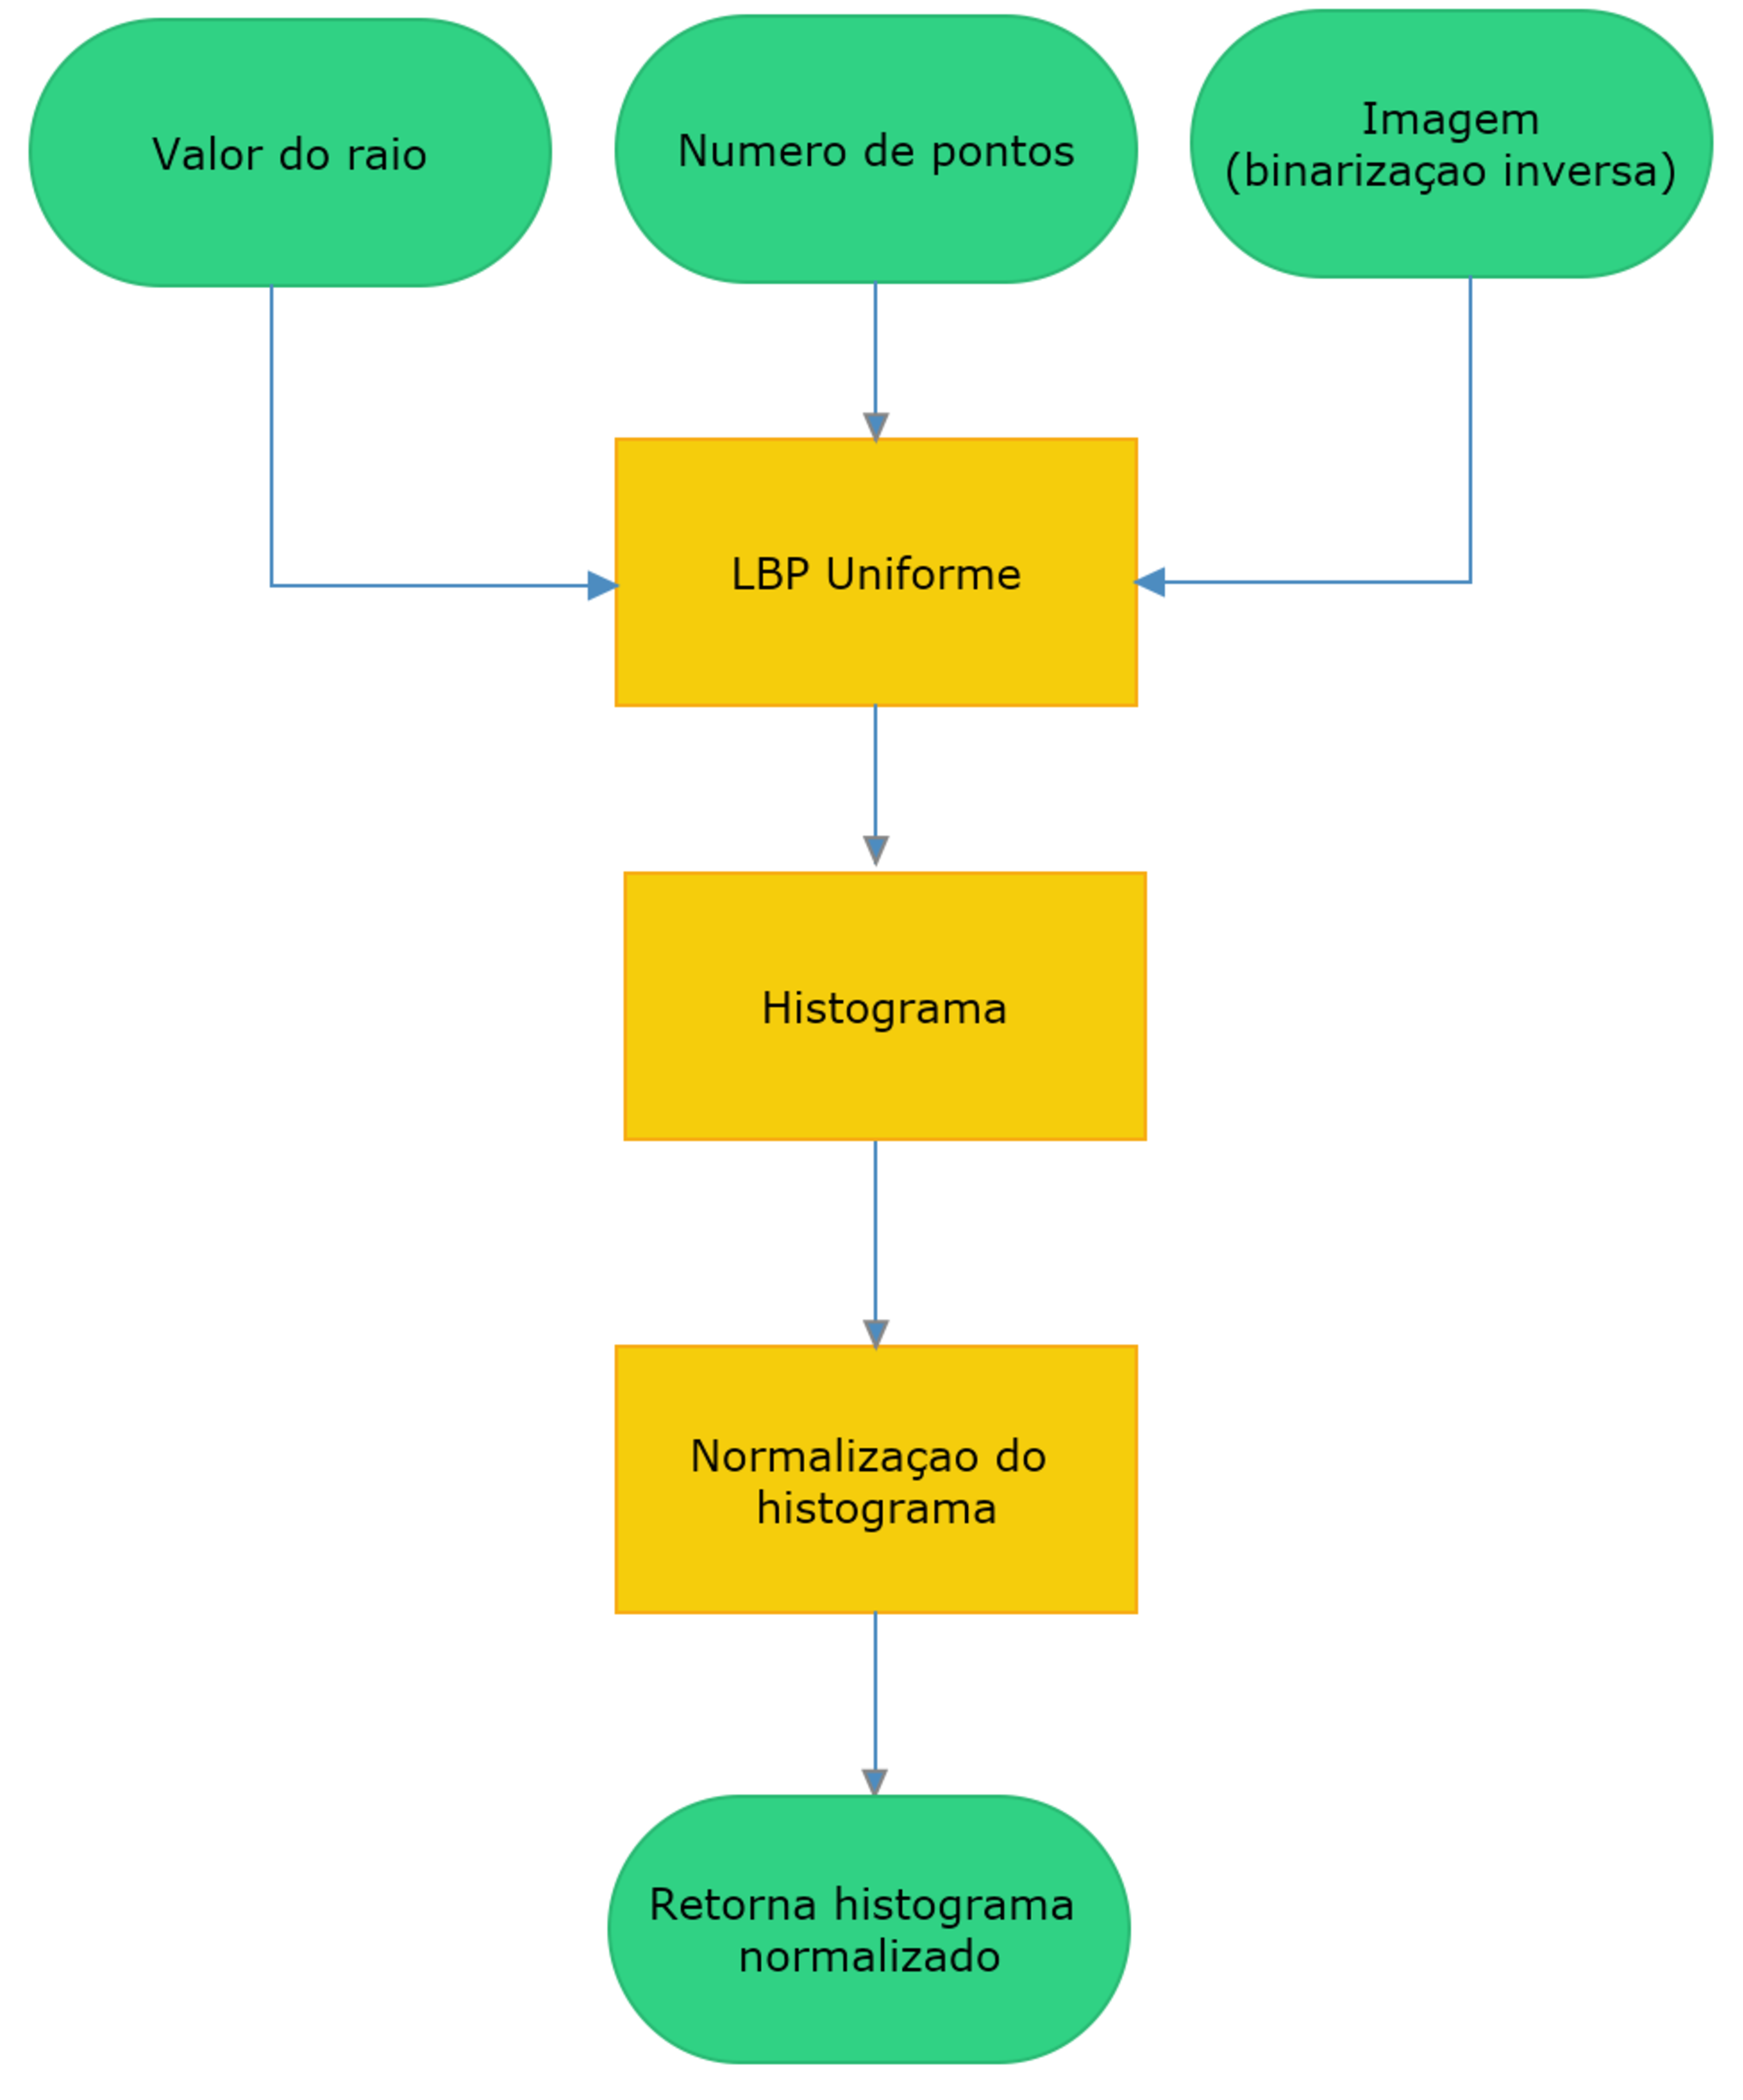
\includegraphics[width=1\linewidth]{figuras/lbp.pdf}
  \caption{Fluxograma do método \texttt{describe} para computar o LBP de uma imagem, retornando seu histograma normalizado.}
  \label{fig:flowLBP}
\end{figure}

Utilizando-se a biblioteca \textit{NumPy} para a estruturação e a manipulação dos vetores de atributos, o histograma da representação da imagem em LBP é então computado e normalizado. O resultado de todo esse processo aplicado às amostras de imagens do banco de imagens é apresentado na Figura \ref{fig:nlbp}. Na Figura \ref{fig:nbinario}, são apresentadas as imagens com binarização inversa, que são as imagens utilizadas como dados de entrada neste estágio (extração de atributos).



A imagem que está sendo analisada segue, então, para a determinação do rótulo referente à sua classe, processo realizado analisando o nome do arquivo. Após isso, o histograma normalizado do LBP, proveniente da extração de atributos, é armazenado em uma lista, denominada Lista de Dados. Em seguida, o rótulo é também armazenado em uma lista, denominada Lista de Rótulos, sendo relacionado ao histograma (representativo dos atributos) por partilharem de mesma posição nas listas de armazanamento. Esse processo é repetido a cada imagem. Toda essa etapa é descrita no fluxograma da Figura \ref{fig:flowtreinamento1}

\begin{figure}[H]
  \centering
  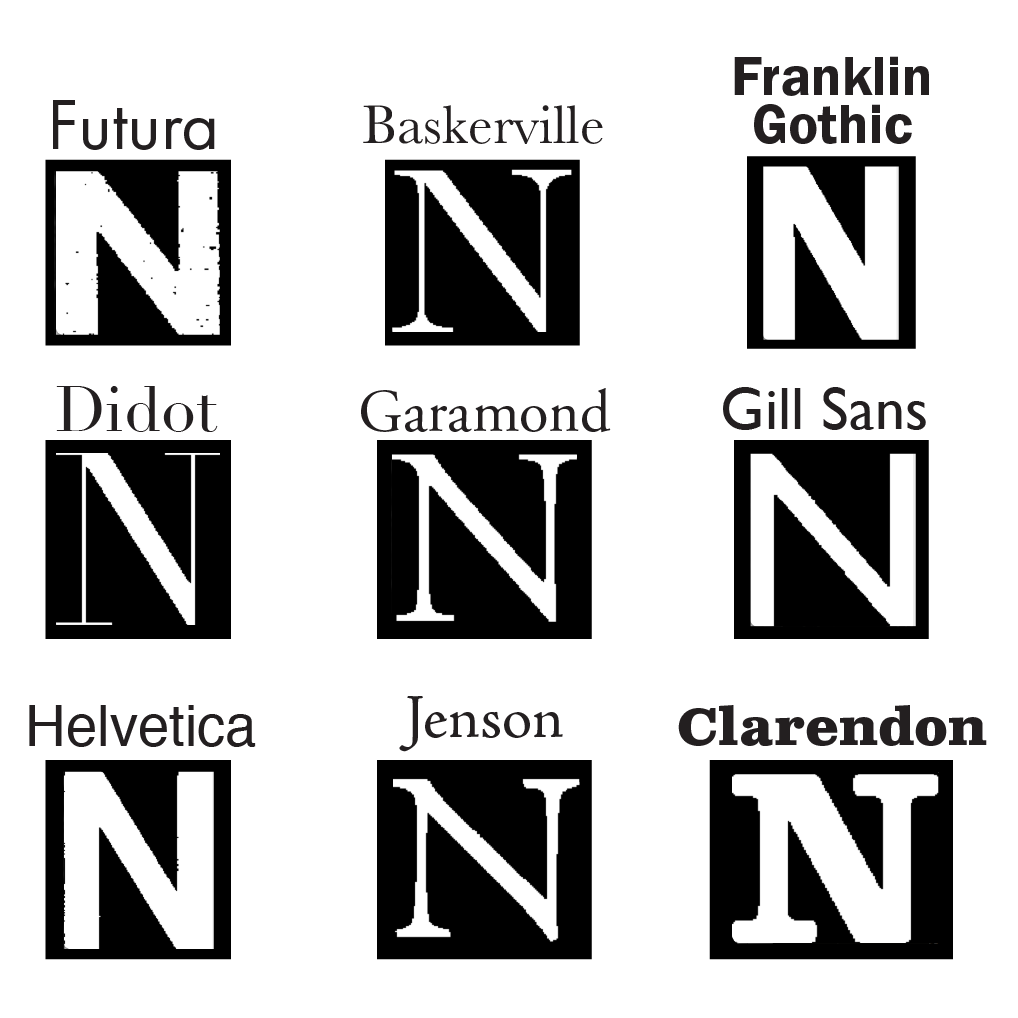
\includegraphics[width=0.4\linewidth]{figuras/nbinario.pdf}
  \caption{Amostras de imagens do banco de imagens após processo de binarização inversa. Imagens de entrada no estágio de extração de atributos.}
  \label{fig:nbinario}
\end{figure}


\begin{figure}[H]
  \centering
  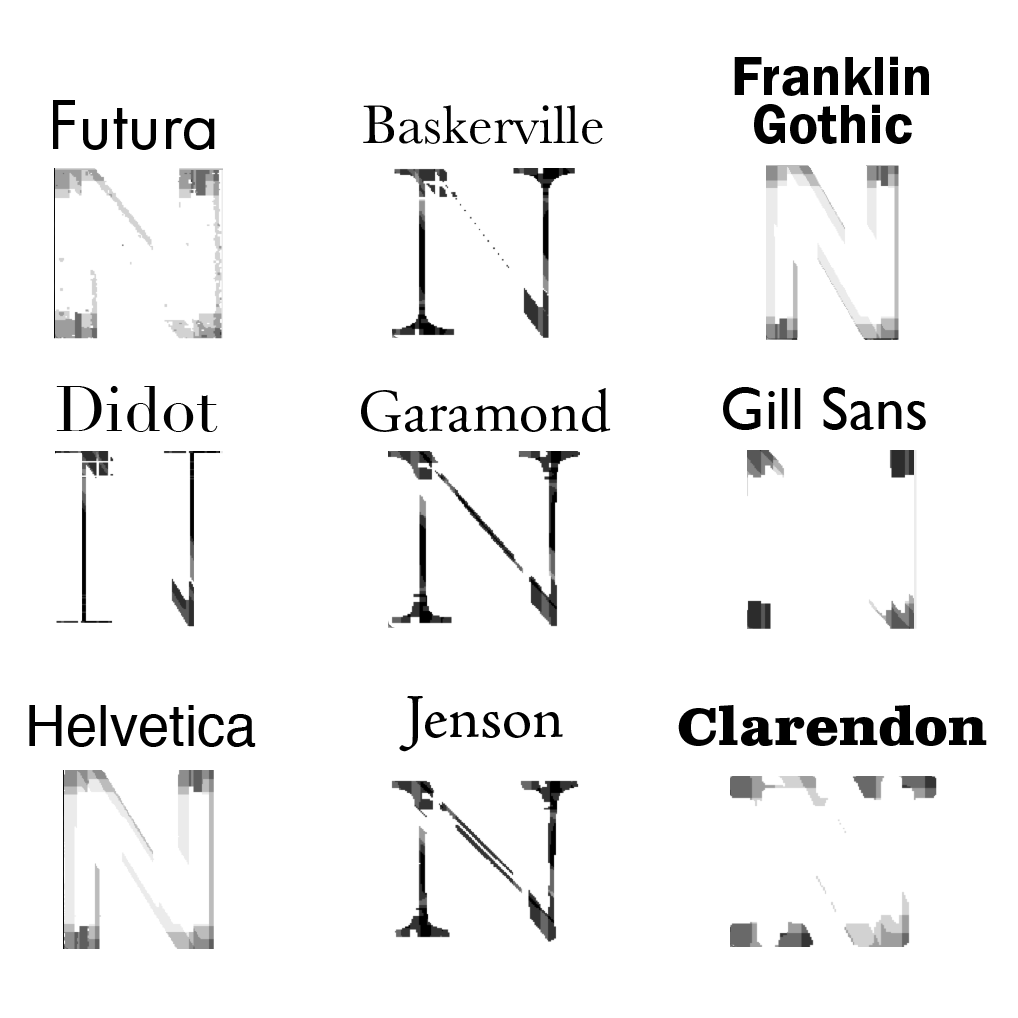
\includegraphics[width=0.4\linewidth]{figuras/enelbp.pdf}
  \caption{Amostras de imagens do banco de imagens após processo de extração de atributos, aplicação do LBP.}
  \label{fig:nlbp}
\end{figure}

Para tornar o processamento mais eficiente, a Lista de Rótulos obtida a partir das imagens é convertida para uma lista formada por inteiros, na qual cada número representa uma classe.

Sendo assim, os elementos de saída deste estágio de extração de atributos são duas listas de dados: uma referente aos rótulos de cada imagem (Lista de Rótulos) e outra, aos histogramas provenientes do LBP (Lista de Dados). São essas duas listas que irão servir de dados de entrada para o estágio de treinamento do modelo.


\begin{figure}[H]
  \centering
  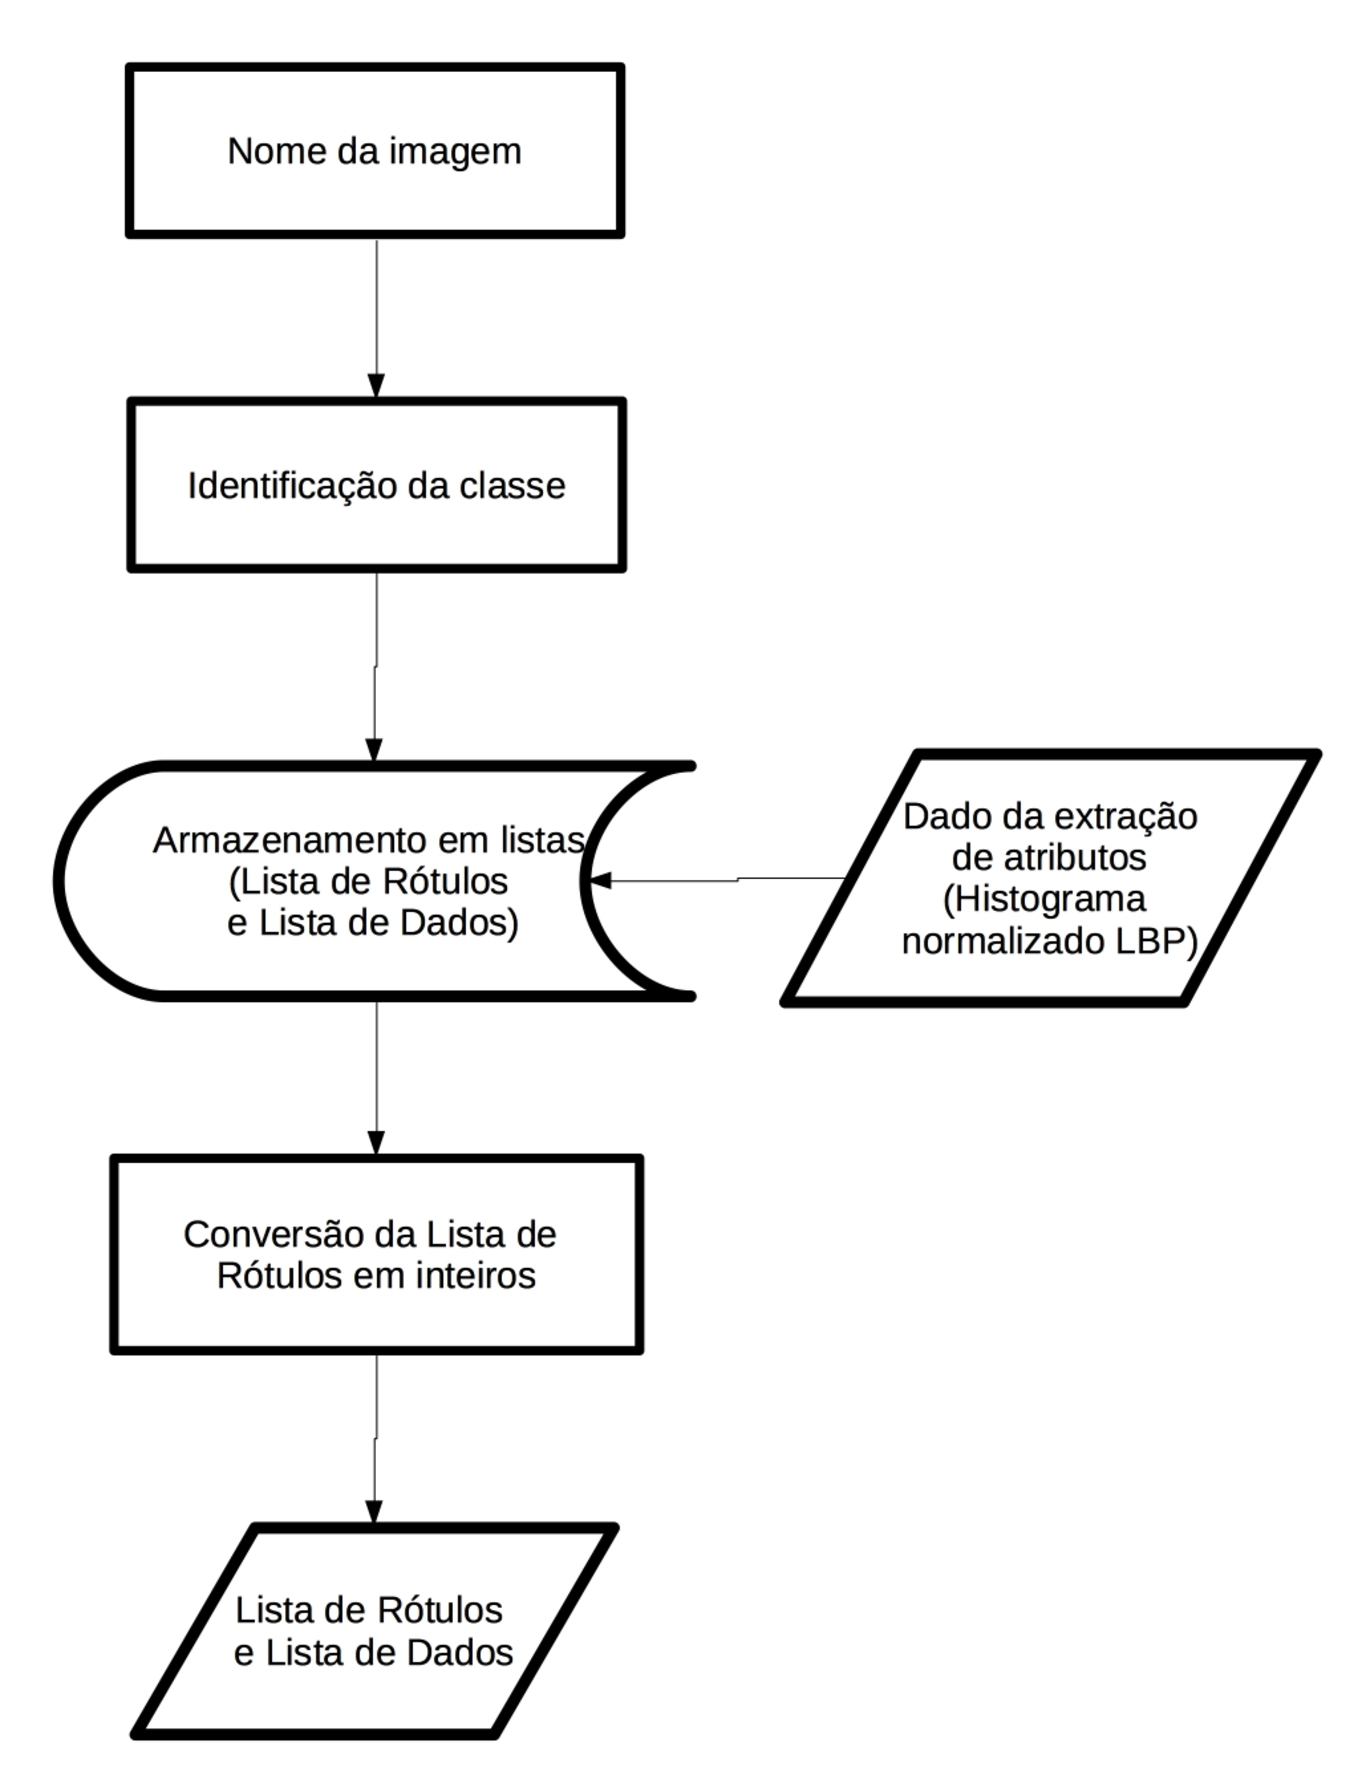
\includegraphics[width=0.55\linewidth]{figuras/treinamento1.pdf}
  \caption{Fluxograma da formação da Lista de Dados e da Lista de Rótulos, ambas dados de entrada para o treinamento do modelo.}
  \label{fig:flowtreinamento1}
\end{figure}


%‘uniform’: improved rotation invariance with uniform patterns and finer quantization of the angular space which is gray scale and rotation invariant.

\subsection{Estágio de treinamento do modelo classificador e testes de predição}

Para o algoritmo desta etapa, a principal biblioteca utilizada foi a \textit{SciKit-learn}, que disponibiliza uma série de ferramentas para várias etapas pertinentes ao aprendizado de máquina. Os módulos utilizados, sendo eles \texttt{svm}, \texttt{ensemble}, \texttt{model\_selection}, \texttt{preprocessing}, oferecem os dois classificadores empregados, métricas para a escolha do modelo e outras ferramentas auxiliares, como a validação cruzada (\textit{Cross Validation}). Todo o processo do estágio de treinamento do classificador e testes de predição é descrito no fluxograma da Figura \ref{fig:flowtreinamento2}.



Nesta etapa, dois modelos foram usados para a classificação das imagens. Primeiramente, utilizou-se o classificador SVM, variando a função \textit{kernel}, a saber, em suas versões Linear, RBF, Sigmoidal e Polinomial. Porém, por apresentar, em todas as alternativas, um índice de acerto de classificação considerado baixo para a aplicação, fato explicitado no próximo capítulo, um novo modelo classificador foi adotado, a Floresta Aleatória.

Para o caso da SVM, foram fornecidos ao modelo alguns parâmetros para sua estruturação, nesse caso, o parâmetro de penalidade \textit{C} do termo erro na classificação, adotado como 100 (o inverso do multiplicador de Lagrange), e o estado randômico (\textit{random state}) para o embaralhamento das imagens, adotado o valor unitário. Além disso, aplicando-se a SVM em uma multiclassificação, utilizou-se a abordagem um-contra-todos, ou seja, são treinados nove classificadores binários, em que uma tipografia é treinada como uma classe e as demais oito tipografias, como a outra classe. Para a classificação de uma nova amostra, são aplicados os nove classificadores binários, aquele que apresenta maior valor, é escolhido como a classe desta imagem.

Para o caso da Floresta Aleatória, os parâmetros fornecidos são o número de árvores de decisão (utilizou-se 82) e o número de tarefas que irão ser realizadas em paralelo (ajustou-se para a execução de número máximo de tarefas em paralelo).

Após isso, passa-se para o ajuste dos parâmetros da validação cruzada a ser utilizada, no caso \textit{Stratified K Fold}. Utilizando essa implementação de validação cruzada, uma variação do modelo \textit{K Fold},  no processo de divisão em subconjuntos (pastas), a porcentagem de amostras de cada classe é mantida de acordo com o conjunto original das imagens. Os parâmetros referentes à validação cruzada utilizada são o número de subconjuntos em que as imagens serão divididas, adotado como sete neste projeto, a opção de embaralhamento e, como no classificador, o estado randômico para o embaralhamento, no qual foi usado valor unitário.

\begin{figure}[H]
 \centering
  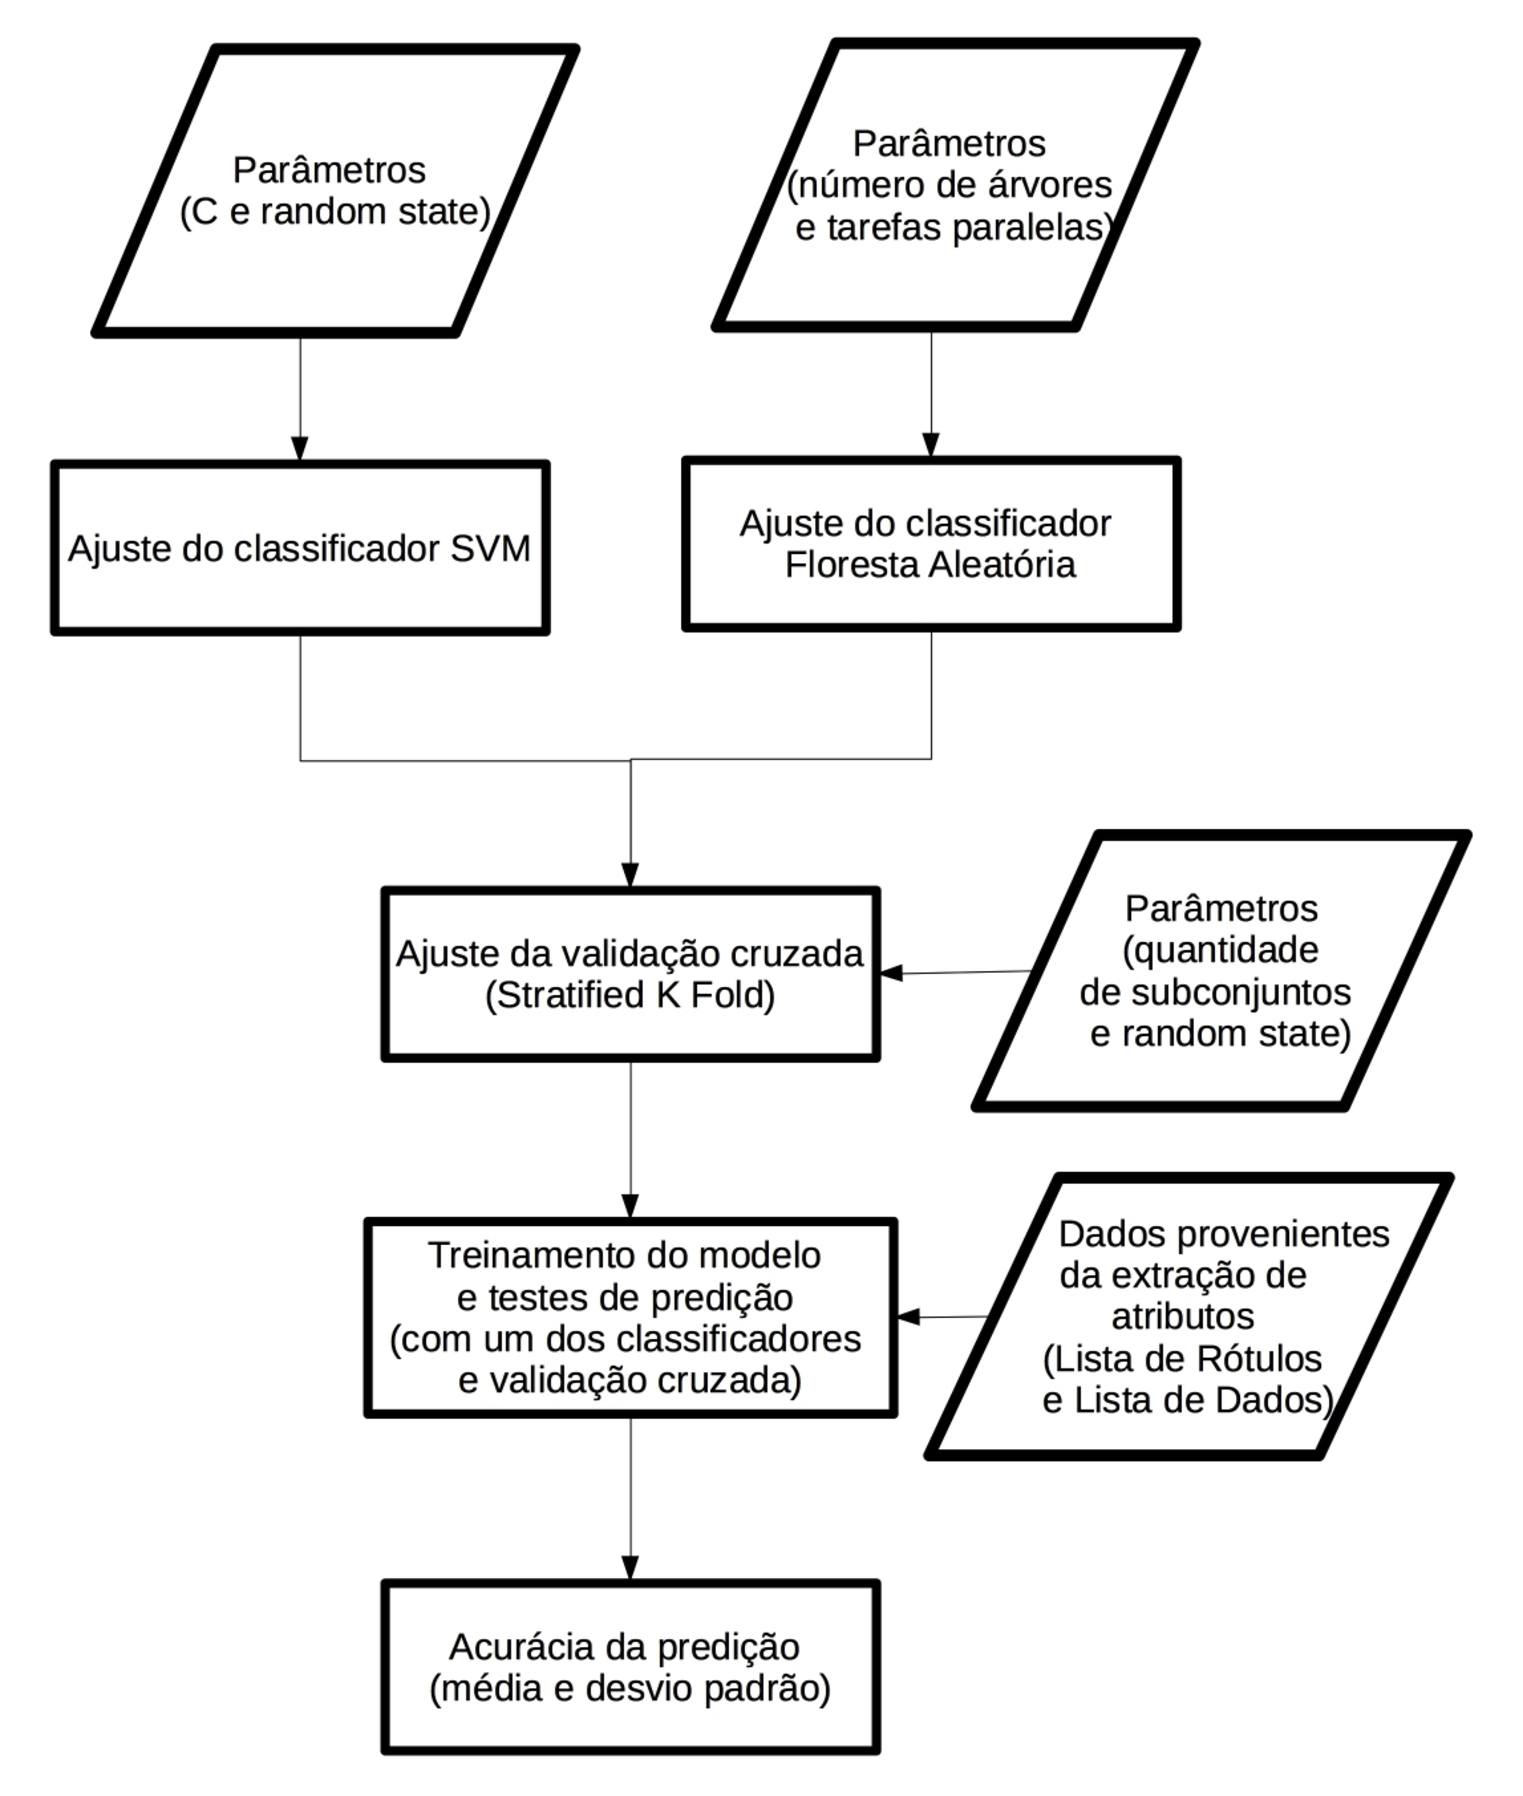
\includegraphics[width=0.6\linewidth]{figuras/treinamento2.pdf}
  \caption{Fluxograma da segunda parte do treinamento do modelo classificador, do ajuste dos modelos classificadores ao resultado de acurácia das predições.}
  \label{fig:flowtreinamento2}
\end{figure}

Em sequência, o classificador é aplicado no conjunto de imagens, o processo se dá com a utilização da validação cruzada previamente ajustada, nesse caso, o treinamento é realizado e, em seguida, o teste da predição. Baseada em todas as iterações da validação cruzada, a acurácia da classificação é calculada, apresentada como a média e o desvio padrão.


Todo o processo descrito nessa seção foi realizado em várias iterações, com a variação de muitos parâmetros que compõem os modelos para que os valores ótimos fossem encontrados. Todos seus resultados serão apresentados no capítulo seguinte.


%metodologia de outro artigo
%The methodology applied in our processing im- age algorithm was based on to estimate features not over full image, instead of this, feature estima- tionwasdoneoverregionsofimagescalled‘‘sub- image’’.Theestimatedattributearraysofeach sub-image were the reference database to recognize thetypeofeachfont(100windowsaretakenran- domlyovereachfulltext) \citeC{aviles2005}


%A \textit{NumPy} foi ainda utilizada no desenvolvimento das duas bibliotecas \textit{SciKit} aqui empregadas. No escopo do algoritmo desenvolvido para o treinamento do modelo de classificação das tipografias, a \textit{NumPy} foi empregue, principalmente, na etapa de pré-processamento e extração de atributos das imagens.



